\documentclass[11pt,a4paper]{article}

\usepackage[utf8]{inputenc}
\usepackage[margin=0.85in]{geometry}
\usepackage{amsmath,amssymb,amsfonts}
\usepackage{graphicx}
\usepackage{xcolor}
\usepackage{subcaption}
\usepackage{float}
\usepackage{hyperref}
\usepackage{listings}
\usepackage{microtype}

% --------------------------------------------------
% Code formatting
% --------------------------------------------------

\definecolor{backcolour}{rgb}{0.96,0.96,0.96}

\lstdefinestyle{console}{
    backgroundcolor=\color{backcolour},
    basicstyle=\ttfamily\small,
    breaklines=true,
    columns=fullflexible,
    keepspaces=true,
    numbers=none,
    frame=single,
    rulecolor=\color{black!20}
}

% --------------------------------------------------
% Hyperlinks
% --------------------------------------------------

\hypersetup{
    colorlinks=true,
    linkcolor=blue!70!black,
    citecolor=blue!70!black,
    urlcolor=blue!70!black
}

% --------------------------------------------------
% Title
% --------------------------------------------------

\title{\textbf{\Large Part 1: Fourier Transform, Frequency-Domain Filtering, and Blurring}}
\author{}
\date{}

\begin{document}

\maketitle

\section{FFT and Inverse FFT Verification}

\subsection{FFT Implementation}

We implemented the radix-2 Cooley--Tukey FFT from scratch. The input is recursively split into its even- and odd-indexed elements and combined using

\[
W_N^k=\exp\left(-\frac{2\pi i k}{N}\right),
\]

\[
X[k]=X_e[k]+W_N^kX_o[k],
\qquad
X[k+N/2]=X_e[k]-W_N^kX_o[k].
\]

The input length must be a power of 2.

\begin{lstlisting}[style=console,caption={Radix-2 1D FFT}]
FFT(x):
    if length(x) == 1:
        return x

    Xe = FFT(even-indexed elements of x)
    Xo = FFT(odd-indexed elements of x)

    for k = 0, ..., N/2 - 1:
        W = exp(-2*pi*i*k/N)
        T = W * Xo[k]

        X[k]       = Xe[k] + T
        X[k + N/2] = Xe[k] - T

    return X
\end{lstlisting}

The inverse FFT was implemented using the same FFT routine:

\[
\operatorname{IFFT}(X)
=
\frac{1}{N}
\overline{\operatorname{FFT}(\overline{X})}.
\]

\subsection{2D FFT}

The 2D FFT was constructed by applying the 1D FFT to every row and then every column:

\[
F(u,v)=
\mathcal{F}_y\left[\mathcal{F}_x[f(x,y)]\right].
\]

The inverse 2D FFT is implemented similarly using the 1D inverse FFT.

\subsection{Image Padding and Verification}

The input photograph was resized so that its longest edge was at most 1024 pixels, giving an image of size

\[
995\times1024.
\]

Since the radix-2 FFT requires power-of-two dimensions, the image was zero-padded to

\[
1024\times1024.
\]

We then computed

\[
f_{\mathrm{reconstructed}}
=
\operatorname{IFFT}(\operatorname{FFT}(f))
\]

and measured the maximum absolute reconstruction error:

\[
E_{\max}
=
\max_{x,y}
\left|f(x,y)-f_{\mathrm{reconstructed}}(x,y)\right|.
\]

The resulting error was

\[
\boxed{E_{\max}=1.136868\times10^{-13}},
\]

which is effectively zero and confirms the correctness of the implementation up to floating-point error.

\begin{figure}[H]
    \centering
    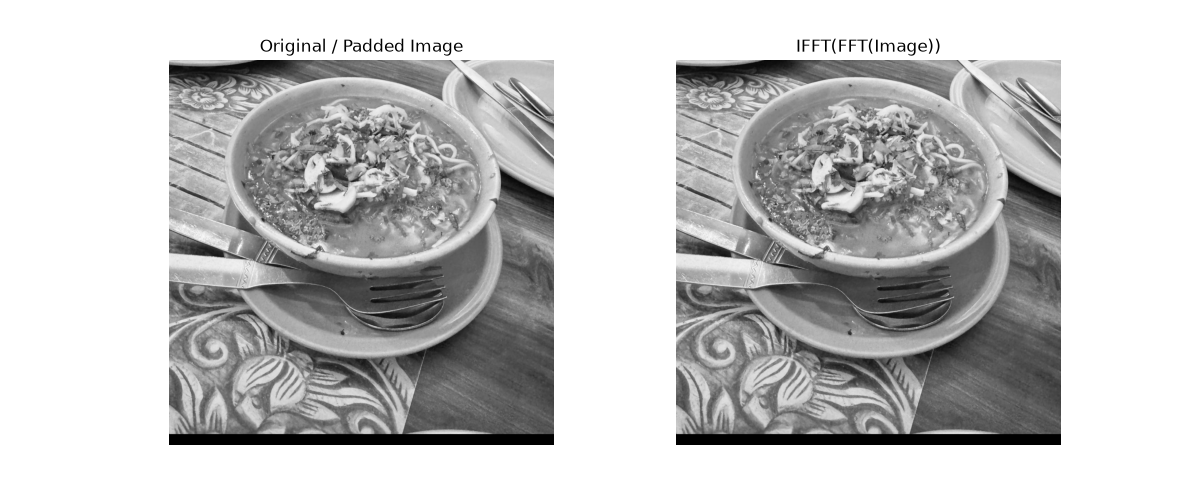
\includegraphics[width=0.8\linewidth]{reconstruction.png}
    \caption{
    FFT verification. Left: original padded image.
    Right: reconstructed image after $IFFT(FFT(\text{Image}))$.
    }
    \label{fig:reconstruction}
\end{figure}


\section{Frequency-Domain Filtering}

We used a normalized $31\times31$ Gaussian kernel to blur the image. By the convolution theorem,

\[
f*h
\quad\longleftrightarrow\quad
F\cdot H,
\]

so the blurred image can be obtained as

\[
g=
\mathcal{F}^{-1}(F\cdot H).
\]

The filtering procedure was:

\begin{enumerate}
    \item Zero-pad the image to $1024\times1024$.
    
    \item Embed the Gaussian kernel in an array of the same size and shift its center to $(0,0)$.
    
    \item Compute the FFTs:
    \[
    F=\mathcal{F}(f),
    \qquad
    H=\mathcal{F}(h).
    \]
    
    \item Multiply them element-wise:
    \[
    G=F\cdot H.
    \]
    
    \item Compute $\mathcal{F}^{-1}(G)$ and crop the result to the original image size.
\end{enumerate}

For visualization, the Fourier spectra were displayed using the log-magnitude

\[
S(u,v)=\log\left(1+|F(u,v)|\right),
\]

with the zero-frequency component shifted to the center.

\begin{figure}[H]
    \centering
    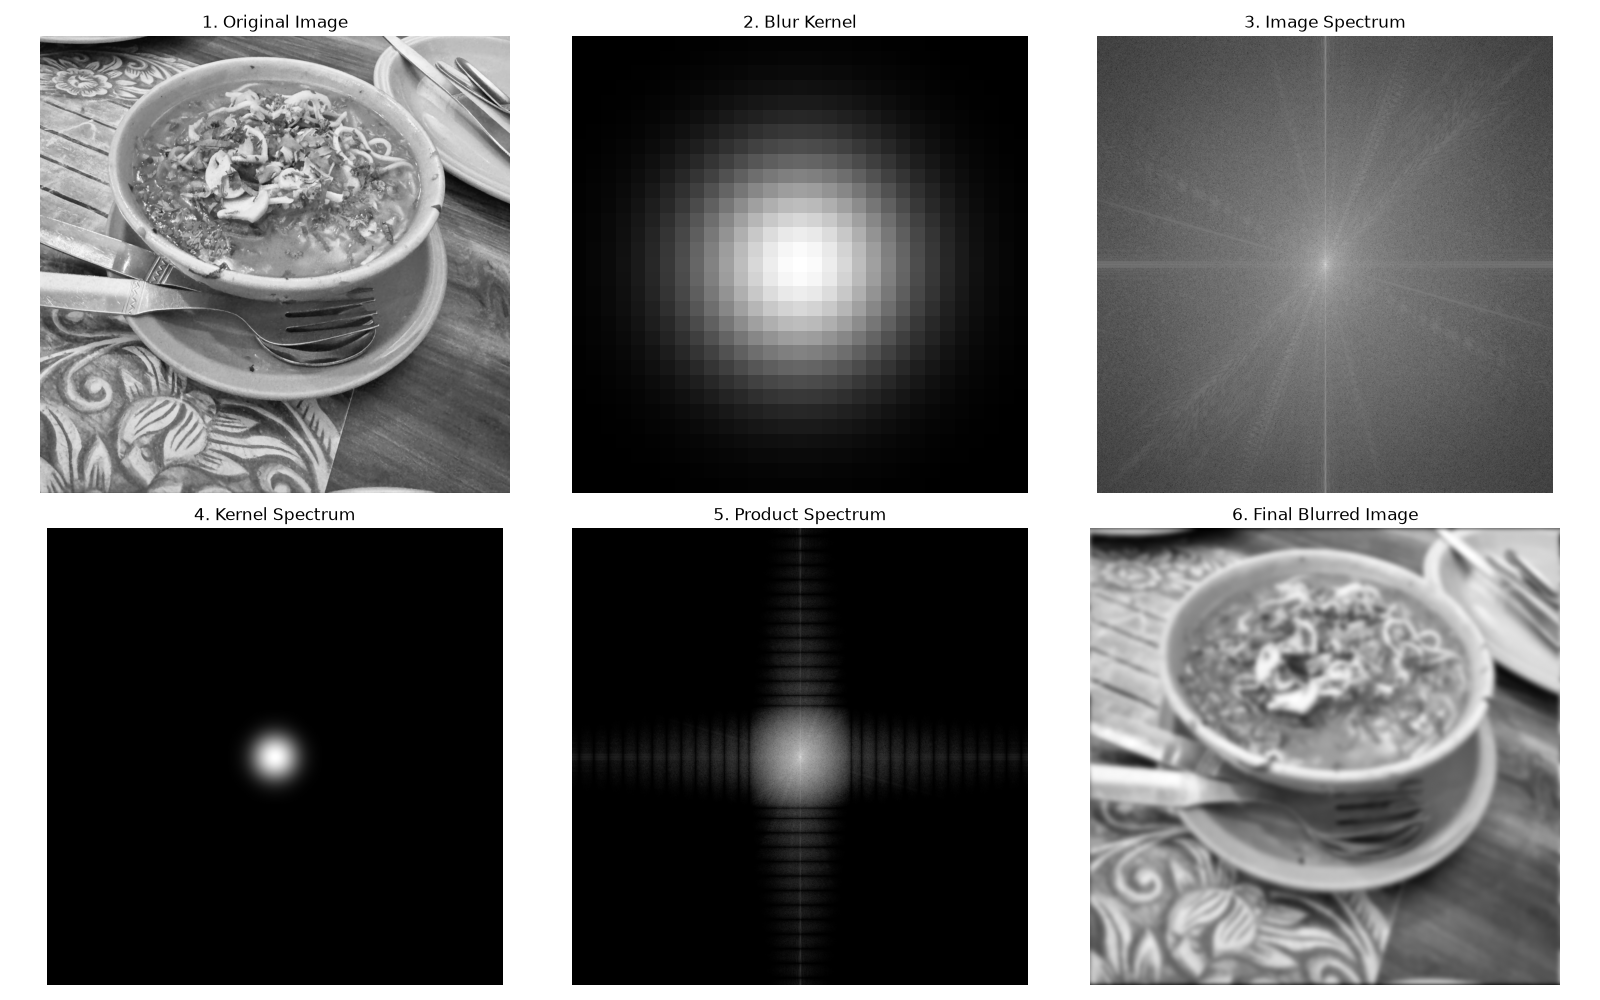
\includegraphics[width=1.0\linewidth]{spectra_steps.png}
    \caption{
    Frequency-domain filtering steps: (1) original padded image,
    (2) Gaussian kernel, (3) image spectrum, (4) kernel spectrum,
    (5) product spectrum, and (6) final blurred image.
    }
    \label{fig:spectra_steps}
\end{figure}

The Gaussian spectrum is concentrated around low frequencies, showing its low-pass behaviour. Multiplication with this spectrum suppresses high-frequency components and produces the blurred image.


\section{Performance Comparison}

\subsection{Experimental Setup}

To compare spatial and frequency-domain filtering, we tested Gaussian kernels of sizes

\[
3,\;31,\;71,\;121,\;201,\;301,\;401,\;501.
\]

A smaller $248\times256$ image was used for timing to keep the computation manageable with our explicit Python FFT implementation.

\subsection{Computational Complexity}

For an $N\times N$ image and an $M\times M$ kernel, direct spatial convolution has complexity

\[
\mathcal{O}(N^2M^2).
\]

The frequency-domain approach requires 2D FFTs with complexity approximately

\[
\mathcal{O}(N^2\log N),
\]

plus element-wise multiplication. For a fixed image size, this cost is largely independent of the kernel size because the kernel is padded to the image dimensions.

\begin{figure}[H]
    \centering

    \begin{subfigure}[b]{0.48\textwidth}
        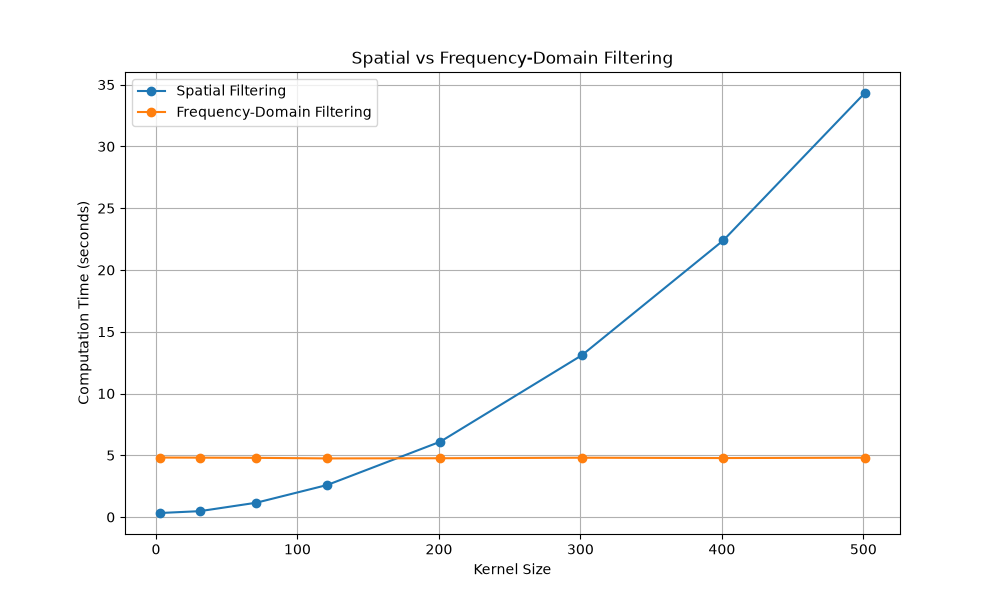
\includegraphics[width=\textwidth]{time_comparison_linear.png}
        \caption{Linear Scale}
    \end{subfigure}
    \hfill
    \begin{subfigure}[b]{0.48\textwidth}
        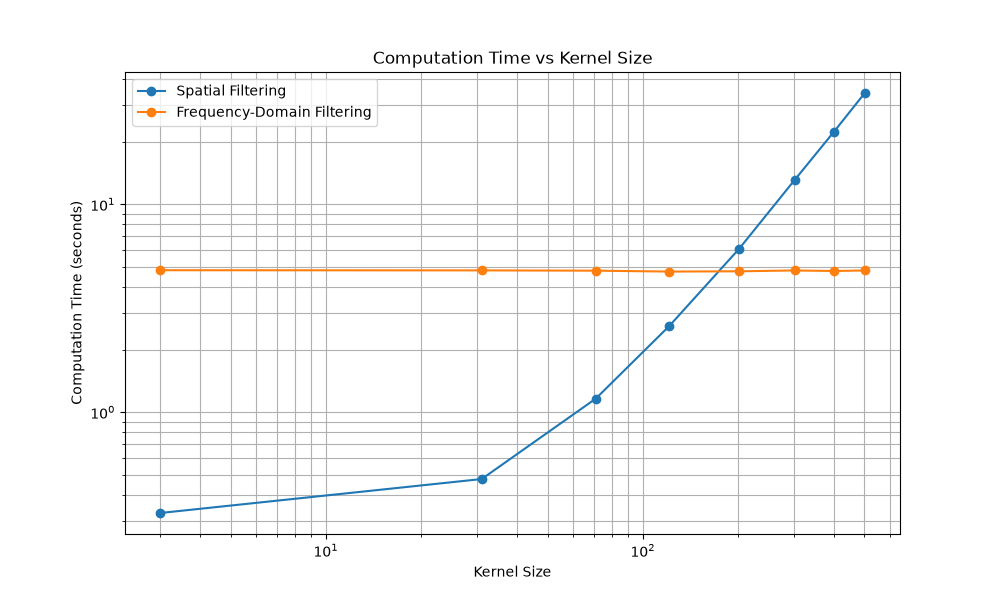
\includegraphics[width=\textwidth]{time_comparison_loglog.png}
        \caption{Log-Log Scale}
    \end{subfigure}

    \caption{
    Computation time versus kernel size for spatial and frequency-domain
    filtering using a $248\times256$ image.
    }
    \label{fig:time_comparison}
\end{figure}

\subsection{Analysis of Performance Results}

The timing results in Figure~\ref{fig:time_comparison} show the different dependence of the two methods on kernel size.

\begin{itemize}
    \item \textbf{Spatial Filtering:}
    The computation time increases rapidly with kernel size because the number of operations per pixel scales as $M^2$. For the tested image, the time increased from approximately $0.08$ seconds for a $3\times3$ kernel to roughly $10$ seconds for a $501\times501$ kernel.

    \item \textbf{Frequency-Domain Filtering:}
    The computation time remains approximately constant at around $1.18$ seconds across the tested kernel sizes. This is because the FFT is performed on the fixed image-sized arrays, regardless of the kernel size.
\end{itemize}

For small kernels, spatial filtering is faster due to the overhead of the FFT. However, as the kernel becomes larger, its quadratic cost causes spatial filtering to become significantly slower. The results therefore demonstrate the advantage of frequency-domain filtering for sufficiently large kernels.


\end{document}